\documentclass[letterpaper]{article}
\usepackage[margin=1in]{geometry}
\usepackage[utf8]{inputenc}
\usepackage{textcomp}
\usepackage{amssymb}
\usepackage{natbib}
\usepackage{graphicx}
\usepackage{gensymb}
\usepackage{amsthm, amsmath, mathtools}
\usepackage[dvipsnames]{xcolor}
\usepackage{enumerate}
\usepackage{mdframed}
\usepackage[most]{tcolorbox}
\usepackage{csquotes}
% https://tex.stackexchange.com/questions/13506/how-to-continue-the-framed-text-box-on-multiple-pages

\tcbuselibrary{theorems}

\newcommand{\R}{\mathbb{R}}
\newcommand{\Z}{\mathbb{Z}}
\newcommand{\N}{\mathbb{N}}
\newcommand{\Q}{\mathbb{Q}}
\newcommand{\C}{\mathbb{C}}
\newcommand{\code}[1]{\texttt{#1}}
\newcommand{\mdiamond}{$\diamondsuit$}
\newcommand{\PowerSet}{\mathcal{P}}
\newcommand{\Mod}[1]{\ (\mathrm{mod}\ #1)}
\DeclareMathOperator{\lcm}{lcm}

%\newtheorem*{theorem}{Theorem}
%\newtheorem*{definition}{Definition}
%\newtheorem*{corollary}{Corollary}
%\newtheorem*{lemma}{Lemma}
\newtheorem*{proposition}{Proposition}


\newtcbtheorem[number within=section]{theorem}{Theorem}
{colback=green!5,colframe=green!35!black,fonttitle=\bfseries}{th}

\newtcbtheorem[number within=section]{definition}{Definition}
{colback=blue!5,colframe=blue!35!black,fonttitle=\bfseries}{def}

\newtcbtheorem[number within=section]{corollary}{Corollary}
{colback=yellow!5,colframe=yellow!35!black,fonttitle=\bfseries}{cor}

\newtcbtheorem[number within=section]{lemma}{Lemma}
{colback=red!5,colframe=red!35!black,fonttitle=\bfseries}{lem}

\newtcbtheorem[number within=section]{example}{Example}
{colback=white!5,colframe=white!35!black,fonttitle=\bfseries}{def}

\newtcbtheorem[number within=section]{note}{Important Note}{
        enhanced,
        sharp corners,
        attach boxed title to top left={
            xshift=-1mm,
            yshift=-5mm,
            yshifttext=-1mm
        },
        top=1.5em,
        colback=white,
        colframe=black,
        fonttitle=\bfseries,
        boxed title style={
            sharp corners,
            size=small,
            colback=red!75!black,
            colframe=red!75!black,
        } 
    }{impnote}
\usepackage[utf8]{inputenc}
\usepackage[english]{babel}
\usepackage{fancyhdr}
\usepackage[hidelinks]{hyperref}
\usepackage{csquotes}

\pagestyle{fancy}
\fancyhf{}
\rhead{Math 170A}
\chead{Monday, February 13, 2023}
\lhead{Lecture 14}
\rfoot{\thepage}

\setlength{\parindent}{0pt}
\newcommand{\0}{\mathbf{0}}
\newcommand{\y}{\mathbf{y}}
\renewcommand{\b}{\mathbf{b}}
\newcommand{\x}{\mathbf{x}}
\newcommand{\e}{\mathbf{e}}
\newcommand{\rr}{\mathbf{r}}
\newcommand{\vv}{\mathbf{v}}
\renewcommand{\u}{\mathbf{u}}

\begin{document}

\section{Condition Numbers \& Perturbation (2.2, 2.3)}
We are now interested in the \emph{sensitivity} of $A\x = \b$ with respect to perturbations (i.e., error). In other words, does noise in $A$ or $\b$ strongly affect the solution $\x$? Here, we'll deal with two types of perturbations: in $\b$, and in $A$. Eventually, we'll talk about the case when there's noise in both. 

\subsection{Motivating Example}
To see what we mean, consider the following two examples.
\begin{mdframed}
    (Example.) Consider the system 
    \[\underbrace{\begin{bmatrix}
        1 & 1 \\ 0 & 1 
    \end{bmatrix}}_A \underbrace{\begin{bmatrix}
        x_1 \\ x_2
    \end{bmatrix}}_{\x} = \underbrace{\begin{bmatrix}
        2 \\ 0
    \end{bmatrix}}_{\b}.\]

    \begin{enumerate}
        \item Solve for $\x$. 
        \begin{mdframed}
            Note that \[\x = \begin{bmatrix}
                2 \\ 0
            \end{bmatrix}\] by backwards substitution.
        \end{mdframed}

        \item Suppose we introduce a very small error to the entries of $\b$ such that $\hat{\b} = \begin{bmatrix}
            2 \\ 0.001
        \end{bmatrix}.$ Our system now becomes \[\underbrace{\begin{bmatrix}
            1 & 1 \\ 0 & 1 
        \end{bmatrix}}_A \underbrace{\begin{bmatrix}
            \hat{x_1} \\ \hat{x_2}
        \end{bmatrix}}_{\hat{\x}} = \underbrace{\begin{bmatrix}
            2 \\ 0.001
        \end{bmatrix}}_{\hat{\b}}.\] Solve for $\hat{\x}$. In other words, what happens to $\x$ if we perturb $\b$?  

        \begin{mdframed}
            Here, we have \[\hat{\x} = \begin{bmatrix}
                1.999 \\ 0.001
            \end{bmatrix}.\]
            Here, $\hat{\x}$ is known as a perturbed solution. Notice how the difference between the solution and the perturbed solution is very small, to the point that both $\x$ and $\hat{x}$ are \emph{similar}.
        \end{mdframed}

        \item Compute the error in $\b$ and in $\x$.
        \begin{mdframed}
            The error in $\b$ can be found by using the $L_2$-norm. So, for $\b$, we have 
            \[||\b - \hat{\b}||_2 = \left|\left| \begin{bmatrix}
                2 \\ 0
            \end{bmatrix} - \begin{bmatrix}
                2 \\ 0.001
            \end{bmatrix} \right|\right|_2 = \left|\left| \begin{bmatrix}
                0 \\ -0.001
            \end{bmatrix} \right|\right|_2 = 0.001\]
            Likewise, for $\x$, we have 
            \[||\x - \hat{\x}||_2 = \left|\left| \begin{bmatrix}
                2 \\ 0
            \end{bmatrix} - \begin{bmatrix}
                1.999 \\ 0.001
            \end{bmatrix} \right|\right|_2 = \left|\left| \begin{bmatrix}
                0.001 \\ -0.001
            \end{bmatrix} \right|\right|_2 = \sqrt{2} \cdot 0.001 \approx 0.0014.\]
        \end{mdframed}
    \end{enumerate}
\end{mdframed}


\begin{mdframed}[nobreak=true]
    (Example.) Consider a similar system 
    \[\underbrace{\begin{bmatrix}
        1 & 1 \\ 0 & 0.001 
    \end{bmatrix}}_A \underbrace{\begin{bmatrix}
        x_1 \\ x_2
    \end{bmatrix}}_{\x} = \underbrace{\begin{bmatrix}
        2 \\ 0
    \end{bmatrix}}_{\b}.\]

    \begin{enumerate}
        \item Solve for $\x$. 
        \begin{mdframed}
            We have 
            \[\x = \begin{bmatrix}
                2 \\ 0
            \end{bmatrix},\] which we found by backwards substitution. 
        \end{mdframed}

        \item Suppose we introduce a very small error to the entries of $\b$ such that $\hat{\b} = \begin{bmatrix}
            2 \\ 0.001
        \end{bmatrix}.$ Our system now becomes \[\underbrace{\begin{bmatrix}
            1 & 1 \\ 0 & 0.001 
        \end{bmatrix}}_A \underbrace{\begin{bmatrix}
            \hat{x_1} \\ \hat{x_2}
        \end{bmatrix}}_{\hat{\x}} = \underbrace{\begin{bmatrix}
            2 \\ 0.001
        \end{bmatrix}}_{\hat{\b}}.\] Solve for $\hat{\x}$.

        \begin{mdframed}
            Here, we have \[\hat{x} = \begin{bmatrix}
                1 \\ 1
            \end{bmatrix}.\]
            One important thing to notice is that the perturbed solution is \emph{quite different} from the actual solution. So, unlike the previous example, $\x$ and $\hat{x}$ are \emph{different}. 
        \end{mdframed}

        \item Compute the error in $\b$ and in $\x$.
        \begin{mdframed}
            The error in $\b$ is the same as in the previous example; therefore,  
            \[||\b - \hat{\b}||_2 = 0.001\]
            But, for $\x$, notice how 
            \[||\x - \hat{\x}||_2 = \left|\left| \begin{bmatrix}
                2 \\ 0
            \end{bmatrix} - \begin{bmatrix}
                1 \\ 1
            \end{bmatrix} \right|\right|_2 = \left|\left| \begin{bmatrix}
                1 \\ -1
            \end{bmatrix} \right|\right|_2 = \sqrt{2} \approx 1.41.\]
            In particular, $0.001$ is $10^3$ larger than 1.41. So, in this linear system, when we perturb $\b$ a little, we can cause a \emph{large} error. 
        \end{mdframed}
    \end{enumerate}
\end{mdframed}

\textbf{Remark:} From this, it follows that the error in $\x$ depends on the matrix $A$ as well. 


\subsection{Condition Number}
How do we measure the dependence on the matrix $A$? This is related to the \textbf{condition number}, known as \code{cond(A)} in MATLAB. The condition number is a simple but useful measure of the sensitivity of the linear system $A\x = \b$. Although we haven't defined the condition number yet, consider the following examples, which showcase the difference in condition number: 
\begin{itemize}
    \item $\cond\left(\begin{bmatrix}
        1 & 1 \\ 0 & 1
    \end{bmatrix}\right) \approx 2.1618$, which is a small condition number. 
    
    \item $\cond\left(\begin{bmatrix}
        1 & 1 \\ 0 & 0.001
    \end{bmatrix}\right) \approx 2 \cdot 10^3$, which is a large condition number, and the error is amplified by this large condition number. 
\end{itemize}

\subsection{Perturbation of \texorpdfstring{$\b$}{b}}
Now, we want to solve $A\x = \b$, where $A$ is invertible. Instead of $\b$, we only have access to \[\hat{\b} = \b + \delta\b,\] where $\delta\b$ is the (very small) error, known as the perturbation in $\b$. Then, we can consider the linear system \[A\hat{\x} = \hat{\b}.\] If $\hat{\b}$ is close to $\hat{\b}$, is it true that $\hat{\x}$ is close to $\hat{\x}$ as well? \textbf{This depends} on the condition number of $A$. In particular, we'll later see that \begin{equation}{\label{2-13:1}}
    \boxed{\frac{||\x - \hat{\x}||}{||\x||} \leq \kappa(A) \frac{||\b - \hat{\b}||}{||\b||}}.
\end{equation} Here, 
\begin{itemize}
    \item $\frac{||\x - \hat{\x}||}{||\x||}$ is the \emph{relative error} of $\x$, 
    \item $\frac{||\b - \hat{\b}||}{||\b||}$ is the \emph{relative error} of $\b$. 
    \item $\kappa(A)$ is the condition number of the invertible matrix $A$.
\end{itemize}
The relative error of $\x$ is bounded by the condition number of matrix $A$ multiplifed by the relative error of $\b$. 

\bigskip 

What is $\kappa(A)$? We can define it like so:  
\[\kappa(A) = ||A|| \cdot ||A^{-1}||,\] where $||\cdot||$ can be any vector norm. We will use the notation 
\begin{itemize}
    \item $\kappa_p$ for the $p$-norm; that is, \[\kappa_{p}(A) = ||A||_p \cdot ||A^{-1}||_p.\]
    \item $\kappa_\infty$ for the $\infty$-norm; that is, \[\kappa_\infty(A) = ||A||_\infty \cdot ||A^{-1}||_\infty.\]
\end{itemize}

With this in mind, let's prove the inequality in (\ref{2-13:1}).
\begin{proof}
    We can break this down into two steps. 
    \begin{itemize}
        \item Let $\hat{\b} = \b + \delta\b$ (the perturbed $\b$) and $\hat{\x} = \x + \delta\x$ (the perturbed $\x$). So, 
        \begin{equation*}
            \begin{aligned}
                A\hat{\x} = \hat{\b} &\implies A(\x + \delta\x) = \b + \delta\b \\ 
                    &\implies A\x + A\delta\x = \b + \delta\b \\ 
                    &\implies A\delta\x = \delta\b && \text{Recall that } A\x = \b \\ 
                    &\implies \delta\x = A^{-1}\delta\b && A \text{ is invertible} \\ 
                    &\implies ||\delta\x|| = ||A^{-1} \delta\b||.
            \end{aligned}
        \end{equation*}
        Recall that $||A|| = \max_{\x \neq \0} \frac{||A\x||}{||\x||}$ is the matrix norm induced by the vector norm. Additionally, note that $||A^{-1}|| = \max_{\x \neq \0} \frac{||A^{-1}\x||}{||\x||}$. Then,
        \[||A^{-1}|| = \max_{\x \neq \0} \frac{||A^{-1}\x||}{||\x||} \geq \frac{||A^{-1}\delta\b||}{||\delta\b||} \implies ||A^{-1}|| \cdot ||\delta\b|| \geq ||A^{-1}\delta\b||.\]
        So, 
        \[||\delta\x|| = ||A^{-1} \delta\b|| \leq ||A^{-1}|| \cdot ||\delta\b|| \implies ||\delta\x|| \leq ||A^{-1}|| \cdot ||\delta\b||.\]

        \item Recall that $\b = A\x$. So, 
        \[\b = A\x \implies ||\b|| = ||A\x|| \leq ||A|| \cdot ||\x||.\]
        Then, we can divide both sides by $||\b|| \cdot ||\x||$ to get 
        \[\frac{1}{||\x||} \leq ||A||\frac{1}{||\b||}.\]
    \end{itemize}
    With all this, we can combine the inequalities
    \[||\delta\x|| \leq ||A^{-1}|| \cdot ||\delta\b||\]
    \[\frac{1}{||\x||} \leq ||A||\frac{1}{||\b||}\]
    to get 
    \[\underbrace{\frac{||\delta\x||}{||\x||}}_{\substack{\text{Relative error} \\ \text{in } \x}} \leq \underbrace{||A^{-1}|| \cdot ||A||}_{\substack{\kappa(A) \\ \text{Condition number.}}} \cdot \underbrace{\frac{||\delta\b||}{||\b||}}_{\substack{\text{Relative error} \\ \text{in } \b}}.\]
   This simplifies to $\frac{||\delta\x||}{||\x||} \leq \kappa(A)\frac{||\delta\b||}{||\b||}$, as desired.  
\end{proof}
\textbf{Remarks:}
\begin{itemize}
    \item The matrix norm is the induced matrix norm, e.g., if the vector norm is 2-norm, then the matrix norm is 2-norm. That is, 
    \[||A||_p = \max_{\x \neq \0} \frac{||A\x||_p}{||\x||_p}\]
    \[||A||_\infty = \max_{\x \neq \0} \frac{||A\x||_\infty}{||\x||_\infty}\]
    This means that we can use whatever vector norm we want for (\ref{2-13:1}) as long as all vectors use the same norm. Additionally, the induced matrix norm for $A$ should be the same as the one used for the vector norm. \textbf{The norms must be consistent in the inequality.}
    \item When interpreting $\kappa(A)$, 
    \begin{itemize}
        \item If $\kappa(A)$ is small (close to 1), then $A$ is called ``well-conditioned.''
        \item If $\kappa(A)$ is large, then $A$ is called ``ill-conditioned.''
    \end{itemize}
    \item A tall matrix does not have a condition matrix because it's not invertible. 
\end{itemize} 

\subsection{Properties of the Induced Matrix Norm}
\begin{proposition}
    Let $||\cdot||$ be an induced matrix norm \[||A|| = \max_{\x \neq \0} \frac{||A\x||}{||\x||}.\] Then, 
    \begin{enumerate}
        \item $||I|| = 1$. Here, $I$ is the identity matrix; the condition number of the identity matrix is 1. 
        \item $\kappa(A) \geq 1$. In particular, the condition number of some matrix will be \emph{at least} 1. 
    \end{enumerate}
\end{proposition}
\begin{proof}
    Note that 
    \[||I|| = \max_{\x \neq \0} \frac{||I\x||}{||\x||} = 1.\]
    Also, 
    \[I = AA^{-1} \implies 1 = ||I|| = ||AA^{-1}|| \leq ||A|| \cdot ||A^{-1}|| = \kappa(A),\]
    so we're done.
\end{proof}

\textbf{Remarks:}
\begin{itemize}
    \item For \#2 of the proposition, if we introduce an error in $\b$, the condition number will not make the error smaller.
    \item $\kappa(I) = 1$. In particular, 
    \[\kappa(I) = ||I|| \cdot ||I^{-1}|| = 1 \cdot 1 = 1.\]
    \item The Feobenius norm is not an induced matrix norm. In particular, the above results do not hold for the Feobenius norm $||I||_F$ as $||I||_F \neq 1$. Recall that 
    \[||A||_F = \sqrt{\sum_{i = 1}^{n} \sum_{j = 1}^{n} (a_{ij})^2}.\]
    However, for $I \in \R^{n \times n}$, 
    \[||I_n||_F = \sqrt{n} \neq 1.\]
\end{itemize}

\subsection{Perturbation of \texorpdfstring{$A$}{A}}
\begin{theorem}{}{}
    Let $A$ be nonsingular, $\b \neq 0$, and let $\x$ and $\hat{\x} = \x + \delta \x$ be solutions to $A\x = \b$ and $(A + \delta A) \hat{\x} = \b$, respectively. Then, 
    \[\frac{||\delta \x||}{||\hat{\x}||} \leq \kappa(A) \frac{||\delta A||}{||A||}.\]
\end{theorem}

\begin{proof}
    We have 
    \begin{equation*}
        \begin{aligned}
            (A + \delta A) \hat{\x} = \b &\implies (A + \delta A) (\x + \delta\x) = \b && \text{We defined } \hat{\x} = \x = \delta\x \\ 
                &\implies A\x + A\delta\x + \delta A\x + \delta A \delta \x = \b \\ 
                &\implies A\x + A\delta\x + \delta A (\x + \delta \x) = \b \\ 
                &\implies A\x + A\delta\x + \delta A \hat{\x} = \b \\ 
                &\implies A\delta\x + \delta A \hat{\x} = \0 && \text{Recall that } A\x = \b \\ 
                &\implies A\delta \x = -\delta A \hat{\x} \\ 
                &\implies \delta\x = -\underbrace{A^{-1}}_{\text{Matrix}} \underbrace{\delta A}_{\text{Matrix}} \underbrace{\hat{\x}}_{\text{Vector}}.
        \end{aligned}
    \end{equation*}
    From here, it follows that
    \begin{equation*}
        \begin{aligned}
            ||\delta\x|| &= ||-A^{-1} \delta A\hat{\x}|| \\ 
                &\leq ||A^{-1}|| \cdot ||\delta A \hat{\x}|| \\ 
                &\leq ||A^{-1}|| \cdot ||\delta A|| \cdot ||\hat{\x}||
        \end{aligned}
    \end{equation*}
    Dividing through by $||\hat{\x}||$, we have 
    \[\frac{||\delta\x||}{||\hat{\x}||} \leq ||A^{-1}|| \cdot ||\delta A||.\]
    Recall that $\kappa(A) = ||A|| \cdot ||A^{-1}|| \implies ||A^{-1}|| = \frac{\kappa(A)}{||A||}$, so 
    \[\frac{||\delta\x||}{||\hat{\x}||} \leq \kappa(A) \frac{||\delta A||}{||A||}\] 
    as desired.
\end{proof}
\textbf{Remark:} $\delta$, in this case, is not a scalar. We can think of $\delta\x$ as $\x$ with a very tiny (and arbitrary) error introduced. Analogously, we can think of $\delta A$ as $A$ with a very tiny (and arbitrary) error. 

\subsection{Perturbation of \texorpdfstring{$A$}{A} and \texorpdfstring{$\b$}{b}}
\begin{theorem}{}{}
    Instead of $A\x = \b$, we now consider $\hat{A}\hat{\x} = \hat{\b}$ with $\hat{A} = A + \delta A$ and $\hat{\b} = \b + \delta\b$. Then, 
    \[\frac{||\delta \x||}{||\hat{\hat{x}}||} \leq \kappa(A) \left(\frac{||\delta A||}{||A||} + \frac{||\delta \b||}{||\hat{\b}||} \cdot \frac{||\delta A||}{||A||} + \frac{||\delta \b||}{||\hat{\b}||}\right)\]
\end{theorem}

\begin{proof}
    We can break this down into two steps.
    \begin{itemize}
        \item For $\hat{A}\hat{\x} = \hat{\b}$, we have 
        \begin{equation*}
            \begin{aligned}
                \hat{A}\hat{\x} = \hat{\b} &\implies (A + \delta A)(\x + \delta \x) = \b + \delta \b \\ 
                    &\implies A\x + A\delta\x + \delta A \x + \delta A \delta \x = \b + \delta \b \\ 
                    &\implies A\delta\x + \delta A \x + \delta A \delta \x = \delta \b && \text{Recall that } A\x = \b \\ 
                    &\implies A\delta\x + \delta A(\x + \delta \x) = \delta \b \\ 
                    &\implies A\delta\x + \delta A\hat{\x} = \delta\b \\ 
                    &\implies A\delta\x = \delta\b - \delta A \hat{\x} \\ 
                    &\implies \delta\x = A^{-1}(\delta \b - \delta A \hat{\x}).
            \end{aligned}
        \end{equation*}
        Now, 
        \begin{equation*}
            \begin{aligned}
                ||\delta\x|| &= ||A^{-1}(\delta \b - \delta A \hat{\x})|| \\
                    &\leq ||A^{-1}|| \cdot ||\delta \b - \delta A \hat{\x}|| \\ 
                    &\leq ||A^{-1}|| (||\delta\b|| + ||\delta A|| \cdot ||\hat{\x}||) && \text{See remark below}.
            \end{aligned}
        \end{equation*}
        Thus, 
        \begin{equation*}
            \begin{aligned}
                ||\delta\x|| &\leq ||A^{-1}|| (||\delta\b|| + ||\delta A|| \cdot ||\hat{\x}||) \\ 
                    &= \frac{||A^{-1}||}{||\hat{\x}||} (||\delta\b|| + ||\delta A|| \cdot ||\hat{\x}||) \\ 
                    &= ||A^{-1}|| \left(\frac{||\delta\b||}{||\hat{\x}||} + \frac{||\delta A|| \cdot ||\hat{\x}||}{||\hat{\x}||}\right) \\ 
                    &= ||A^{-1}|| \left(\frac{||\delta\b||}{||\hat{\x}||} + ||\delta A||\right) \\ 
                    &= \frac{\kappa(A)}{||A||} \left(\frac{||\delta\b||}{||\hat{\x}||} + ||\delta A||\right) && \kappa(A) = ||A|| \cdot ||A^{-1}|| \implies ||A^{-1}|| = \frac{\kappa(A)}{||A||} \\ 
                    &= \kappa(A) \left(\frac{||\delta\b||}{||A|| \cdot ||\hat{\x}||} + \frac{||\delta A||}{||A||}\right).
            \end{aligned}
        \end{equation*}

        \item Again, from $\hat{A}\hat{\x} = \hat{\b}$, we have 
        \[\hat{A}\hat{\x} = \hat{\b} \implies (A + \delta A) \hat{\x} = \hat{\b}.\]
        Then, 
        \[||\hat{\b}|| = ||(A + \delta A) \hat{\x}|| \leq ||A + \delta A|| \cdot ||\hat{\x}||.\]
        Therefore, dividing by $||\hat{\x}|| \cdot ||\hat{\b}||$ we get 
        \[\frac{1}{||\hat{\x}||} \leq \frac{||A + \delta A||}{||\b||} \leq \frac{||A|| + ||\delta A||}{||\delta \b||}.\]
    \end{itemize}
    Combining the results of the previous two steps yields the desired result.
\end{proof}

% \begin{equation*}
%     \begin{aligned}
%         ||\delta\x|| \frac{1}{||\hat{\x}||} &\leq \kappa(A) \left(\frac{||\delta\b||}{||A|| \cdot ||\hat{\x}||} + \frac{||\delta A||}{||A||}\right) \frac{||A|| + ||\delta A||}{||\delta \b||} \\ 
%             &= \kappa(A) \left(\frac{||\delta\b||}{||A|| \cdot ||\hat{\x}||} \frac{||A|| + ||\delta A||}{||\delta \b||} + \frac{||\delta A||}{||A||} \frac{||A|| + ||\delta A||}{||\delta \b||}\right) \\ 
%             &= \kappa(A) \left(\frac{||\delta \b||(||A|| + ||\delta A||)}{||A|| \cdot ||\hat{\x}|| \cdot ||\delta \b||} + \frac{||\delta A||(||A|| + ||\delta A||)}{||A|| \cdot ||\delta \b||}\right) \\
%             &= \kappa(A) \left(\frac{||\delta \b|| \cdot ||A|| + ||\delta \b|| \cdot ||\delta A||}{||A|| \cdot ||\hat{\x}|| \cdot ||\delta \b||} + \frac{||\delta A|| \cdot ||A|| + ||\delta A|| \cdot ||\delta A||}{||A|| \cdot ||\delta \b||}\right) \\
%             &= \kappa(A) \left(\frac{||\delta \b|| \cdot ||A||}{||A|| \cdot ||\hat{\x}|| \cdot ||\delta \b||} + \frac{||\delta \b|| \cdot ||\delta A||}{||A|| \cdot ||\hat{\x}|| \cdot ||\delta \b||} + \frac{||\delta A|| \cdot ||A||}{||A|| \cdot ||\delta \b||} + \frac{||\delta A|| \cdot ||\delta A||}{||A|| \cdot ||\delta \b||}\right) \\
%             &= \kappa(A) \left(\frac{1}{||\hat{\x}||} + \frac{||\delta A||}{||A|| \cdot ||\hat{\x}||} + \frac{||\delta A||}{||\delta \b||} + \frac{||\delta A|| \cdot ||\delta A||}{||A|| \cdot ||\delta \b||}\right) \\
%     \end{aligned}
% \end{equation*}

\textbf{Remark:} To see why this equality works, consider the following diagram:
\begin{center}
    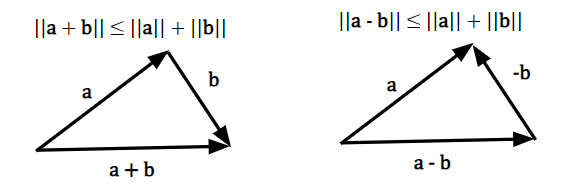
\includegraphics[scale=0.8]{../assets/triangle_min_plu.png}
\end{center}




\end{document}